\documentclass[aspectratio=169]{beamer}


\usepackage[utf8]{inputenc}
\usepackage{amsmath}
\usepackage{amsfonts}
\usepackage{amssymb}
\usepackage{graphicx}
\usepackage{ragged2e}  % `\justifying` text
\usepackage{booktabs}  % Tables
\usepackage{tabularx}
\usepackage{tikz}      % Diagrams
\usetikzlibrary{calc, shapes, backgrounds}
\usepackage{amsmath}
\usepackage{amssymb}
\usepackage{dsfont}
\usepackage{url}       % `\url
\usepackage{listings}  % Code listings
\usepackage[T1]{fontenc}
\usepackage{subcaption}
\usepackage[table]{xcolor}
\usepackage{hyperref}
\usepackage{pdflscape}
\usepackage{graphicx}

\usepackage{theme/beamerthemehbrs}

\author[Name]{Linta Mariya Joy}

%\title{Machine Learning-Based Prediction of SASA  from Partial Molecular Dynamics Simulations for Comparative Analysis of Molecular Systems}
\title{Machine Learning Prediction of Structural Dynamics and Molecular Properties from Partial Molecular Dynamics Simulations in Cyclodextrin–Drug Systems}
\institute[HBRS]{Hochschule Bonn-Rhein-Sieg}
\date{\today}

% leave the value of this argument empty if the advisors
% should not be included on the title slide
\def\advisors{Dr. Hebah Fatafta}

% \thirdpartylogo{path/to/your/image}

\begin{document}
{
\begin{frame}

\titlepage
\end{frame}
}

\begin{frame}{Project Overview}
\begin{figure}
    \centering
    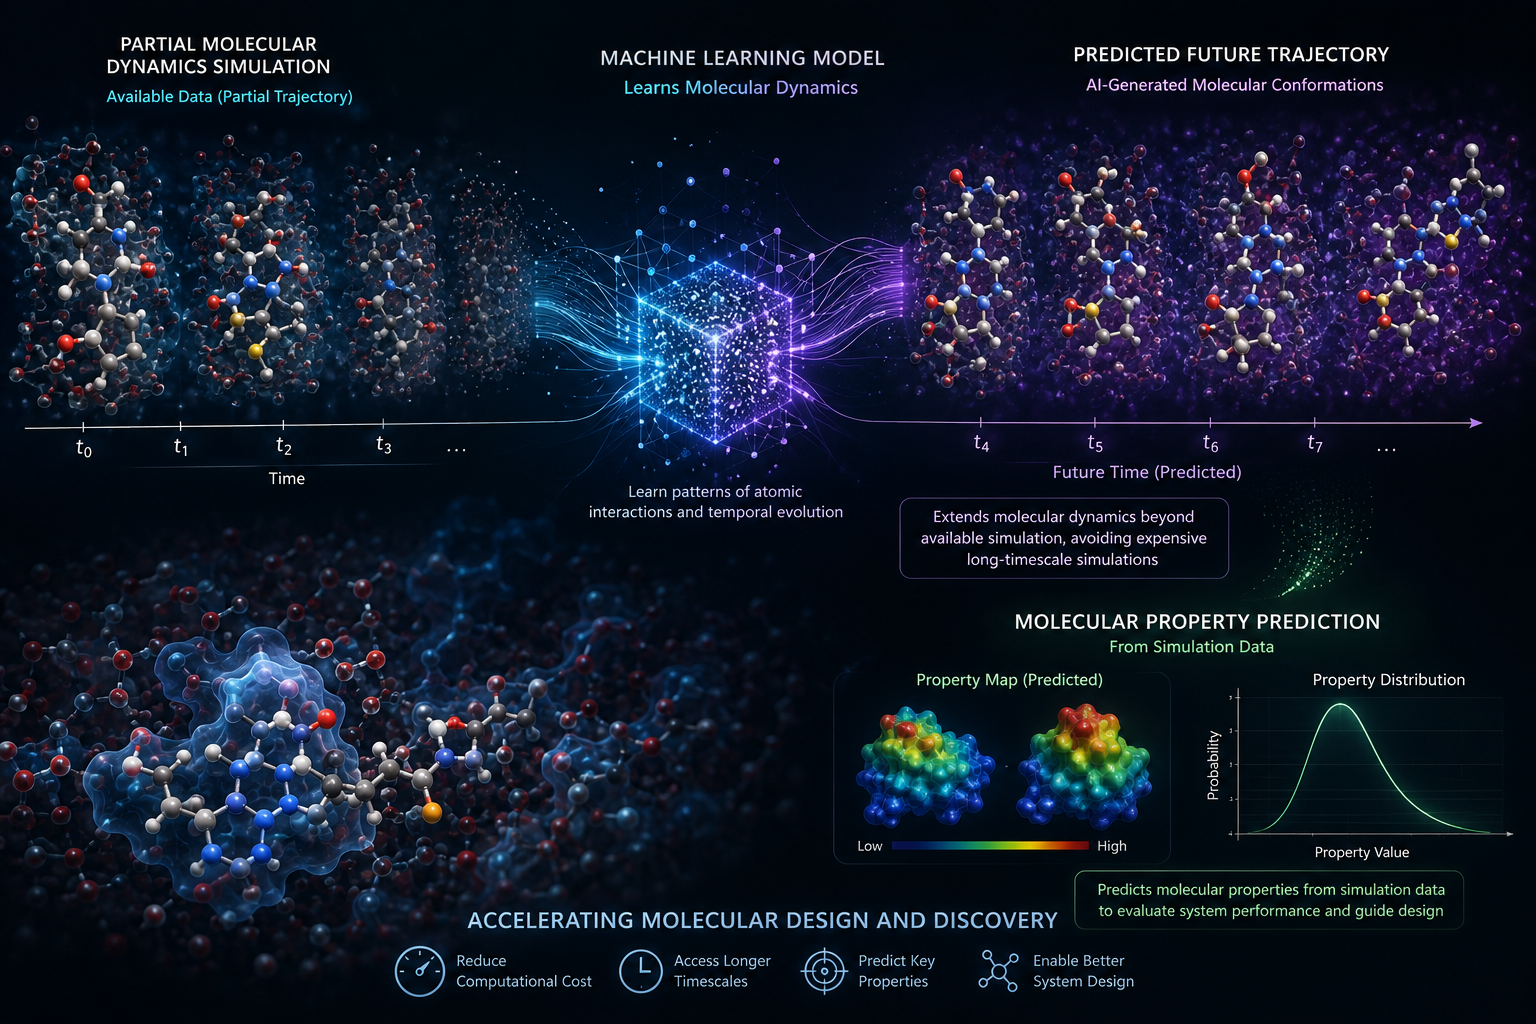
\includegraphics[width=14cm, height = 5.8cm ]{theme/images/project_overview.png}
    \caption{Project Overview ( \url{https://chatgpt.com/})} 
    
\end{figure}


\end{frame}

\begin{frame}{System}
Applied to \textbf{cyclodextrin} inclusion complex systems, which are important in drug delivery for improving solubility and stability
    \begin{figure}
        \centering
        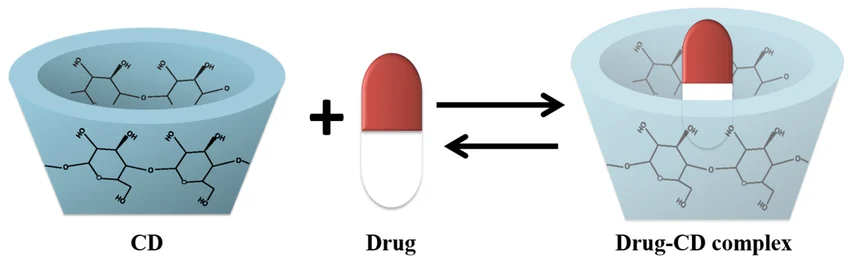
\includegraphics[width=0.85\linewidth]{theme/images/Cyclo_drug_1.pdf}
        \caption{Cyclodextrin-drug}
        %\label{fig:placeholder}
    \end{figure}
\end{frame}

%cyclodextrin inclusion complex systems are important in drug delivery for improving solubility and stability
%Drug–host interactions depend on structural dynamics and exposure behavior
%molecular dynamics simulation provides detailed insights but is computationally expensive
%Long simulations and multiple system comparisons are difficult to scale
%Machine learning with structural descriptors (MBTR) can approximate structure–property relationships efficiently
%Enables faster prediction of structural evolution and properties like solvent accessible surface area
\begin{frame}{Motivation}
    \begin{tikzpicture}[overlay,remember picture]
        \node[anchor=south east,xshift=-30pt,yshift=35pt]
          at (current page.south east) {
            %\includegraphics[width=35mm]{resources/jabberwocky-light}
          };
%HF: Too much text, also beynod motivation there should be one slide tell what is big picture vision, i.e. integrate ML with MD (surrogate??). Then comes your motivation
% In general for all your slides, shorten the pullet points
% You have to think of the remaining points after point 4
%
      \end{tikzpicture}%
      \begin{itemize}
        %\item Study molecular dynamics (MD).
        %\item Large trajectory datasets.
        %\item Computationally expensive simulations.
        %\item SASA quantifies solvent exposure.
        %\item Model structure–SASA relationships.
        %\item Predict future trajectory behavior.
        %\item cyclodextrin inclusion complex systems are important in drug delivery for improving solubility and stability
        \item Drug–host interactions depend on structural dynamics and exposure behavior
        \item MD simulation provides detailed insights but is computationally expensive
        \item ML with structural descriptors (MBTR) can approximate structure–property relationships efficiently
        \item Enables faster prediction of structural evolution and properties like solvent accessible surface area
        
      \end{itemize}
      
\end{frame}

\begin{frame}{Literature Review}

\begin{table}[ht]
\centering

\footnotesize
\large
\resizebox{15cm}{!}{
\begin{tabular}{|>{\centering\arraybackslash}p{2.3cm}|>{\raggedright\arraybackslash}p{5.5cm}|>{\raggedright\arraybackslash}p{5.5cm}|>{\raggedright\arraybackslash}p{5.6cm}|}
\hline
\textbf{Aspect} & \textbf{Kibria et al. (2023)} & \textbf{Han et al. (2023)} & \textbf{Jahandoost et al. (2024)} \\
\hline
System & Gold-core NPs, 9 drug types & Liposome formulations & Same NP dataset as Kibria \\
\hline
Target & SASA & Size, PDI, zeta, encapsulation & SASA \\
\hline
Data & 119 MD-simulated NP designs & 665 experimental liposome formulations & Same 119 NP designs (reused) \\
\hline
Descriptor & MBTR (72 features) & Molecular/process descriptors & MBTR (72 features) \\
\hline
ML models & Transformer/XGBoost + DNN & LightGBM, RF, SVM, PLS, MLR & Linear Regression + Extra Trees \\
\hline
Key method & MBTR forecast $\to$ DNN SASA + SHAP & Best ML per parameter + CG-MD check & LR forecast $\to$ augmentation $\to$ ETR \\
\hline
Best result & MAE 1.57; 7.5$\times$ faster than MD & $R^2$=0.83 (size), 0.76 (zeta) & 25\% more accurate, 40$\times$ faster than Kibria \\
\hline
\end{tabular}
}
\caption{Literature review summary of ML/MD approaches for nanocarrier drug delivery design}
\label{tab:lit_review}
\end{table}
\end{frame}



\begin{frame}{Research Objectives}
To assess whether MBTR-based ML models can predict future structural states and (SASA?) of cyclodextrin–drug systems and generalize across multiple configurations.\\
To do so we need to develop pipline:\\

     \begin{itemize}
         \item Extract MBTR $\&$ Compute SASA from MD data
         %\item Compute SASA
         \item Build Machine Learning Models
         \item MBTR Timeseries Prediction/SASA Prediction
         %\item SASA Prediction
         \item Compare different systems based on error value
     \end{itemize}
\end{frame}


\begin{frame}{Pipeline}
  \begin{figure}
      \centering
      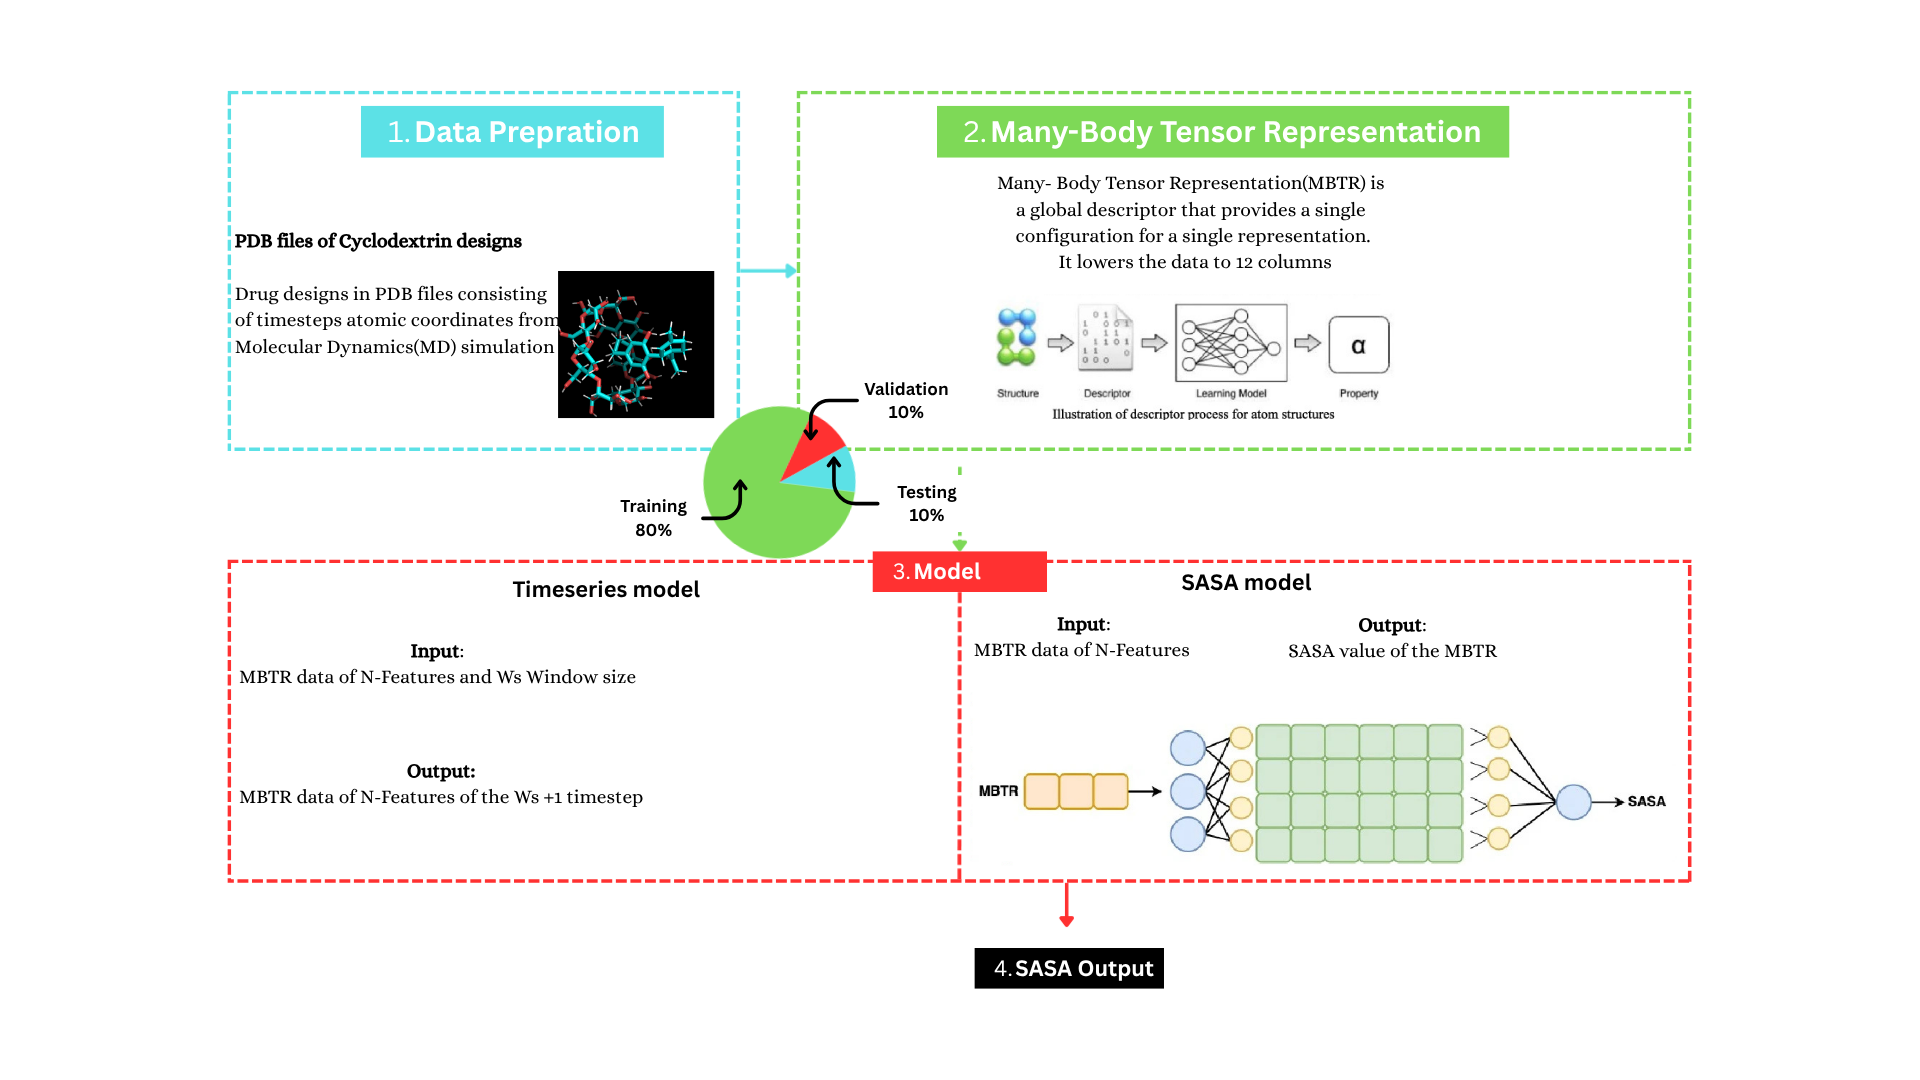
\includegraphics[width=16cm, height =6cm]{theme/images/Add a little bit of body text.png}
      \caption{Pipeline}
      \label{fig:placeholder}
  \end{figure}
\end{frame}

\begin{frame}{Raw Data}

\begin{columns}

% LEFT SIDE: TEXT
\begin{column}{0.5\textwidth}
\begin{itemize}
    \item 4 CD–CBD binding systems
    \item 200 ns MD simulations each
    \item Distinct binding orientations explored
\end{itemize}
\end{column}

% RIGHT SIDE: IMAGE
\begin{column}{0.5\textwidth}
\centering
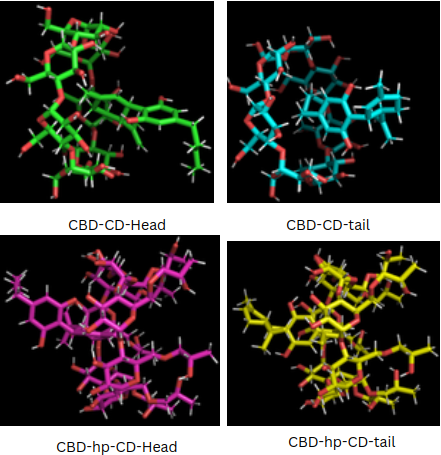
\includegraphics[width=\linewidth]{theme/images/Systems.png}
\captionof{figure}{Cyclodextrin–CBD systems overview}
\end{column}

\end{columns}

\end{frame}


\begin{frame}{Data Prepration}
    \begin{figure}
        \centering
        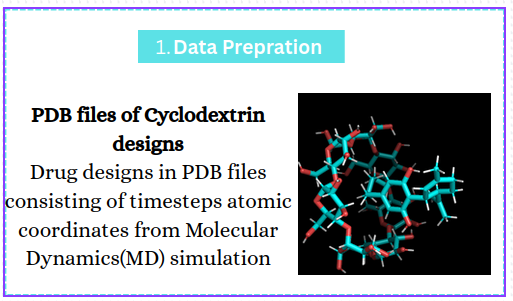
\includegraphics[width=10cm, height =6cm]{theme/images/data_prepration.png}
        \caption{Data Prepration}
        \label{fig:placeholder}
    \end{figure}
\end{frame}

%HF: MBTR definition
% MBTR is a global descriptor that maps a molecular configuration to a fixed-length numerical vector, enabling machine learning models to learn structure–property relationships from atomistic data

% Simplified one: MBTR = a way to turn a whole molecule (geometry + composition) into numbers that ML can understand.

\begin{frame}{Many Body Tensor Representation}
    \begin{figure}
        \centering
        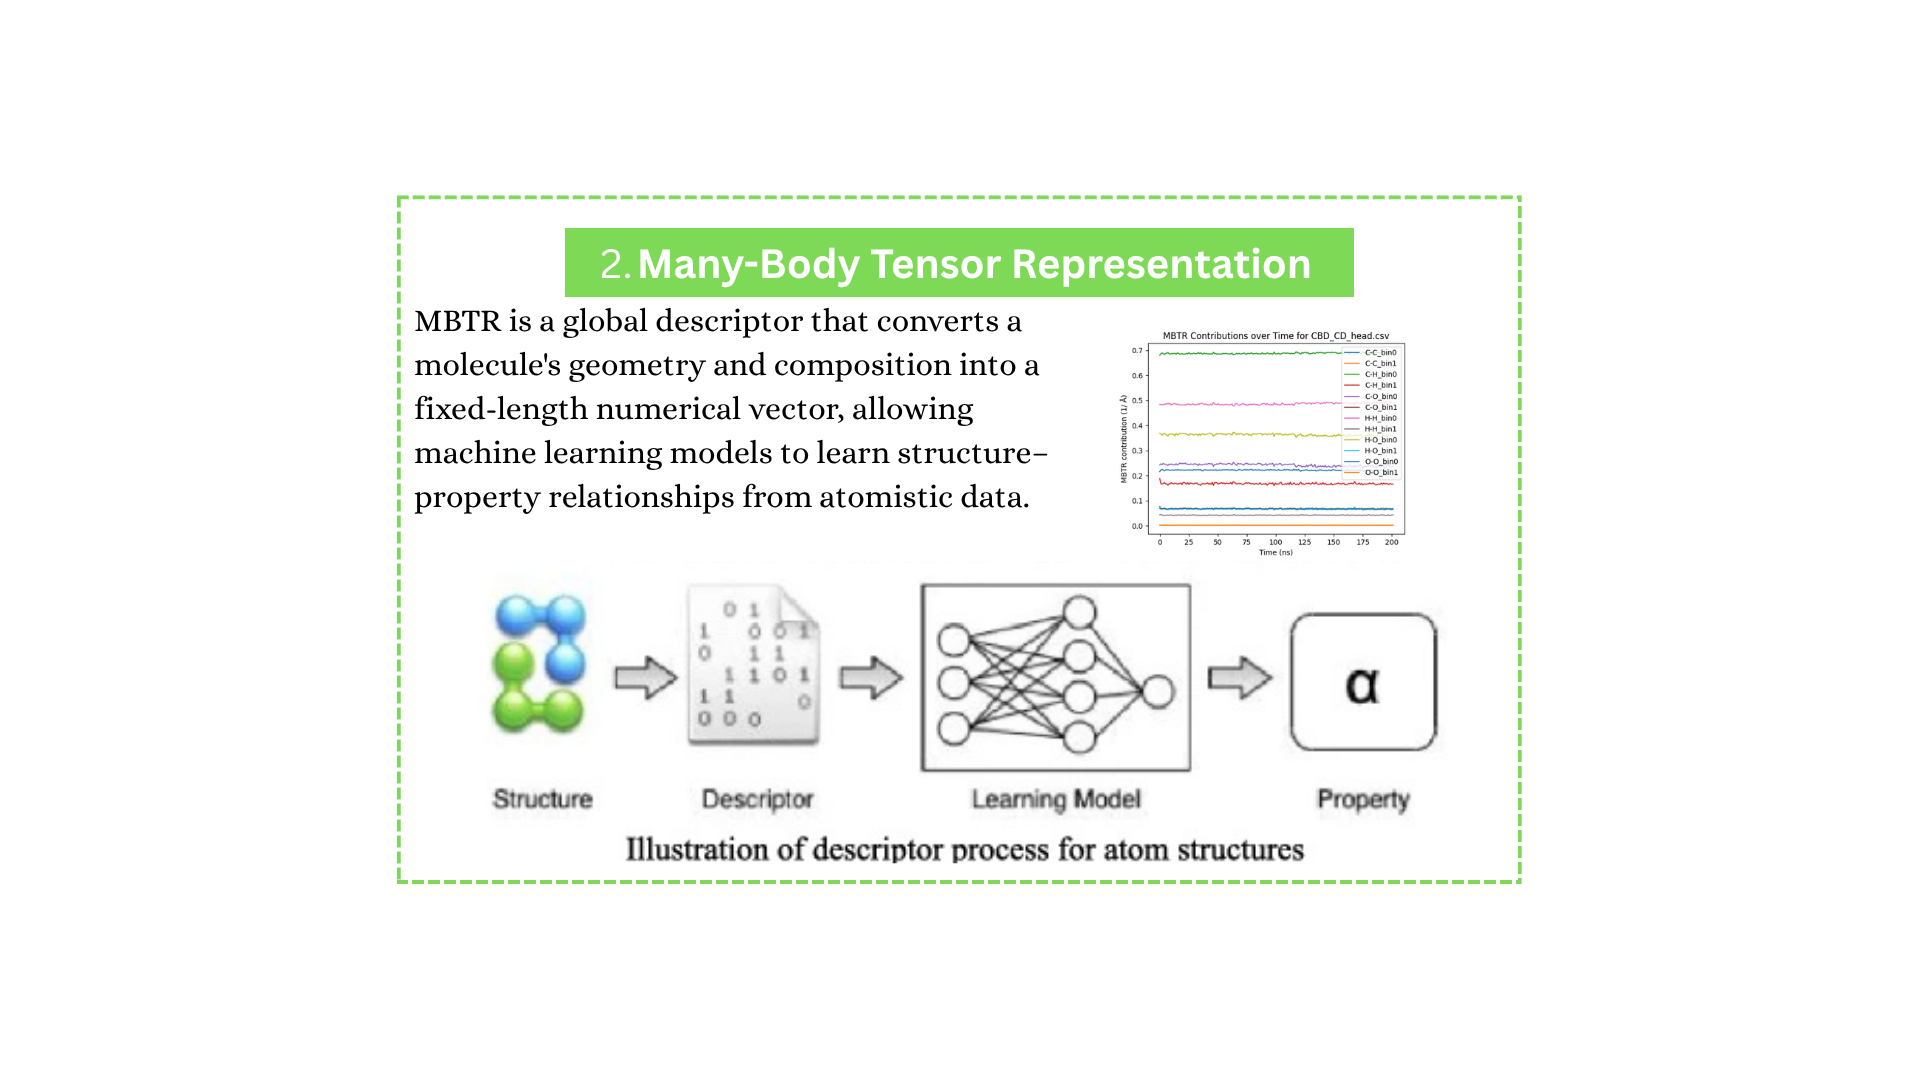
\includegraphics[width=12cm, height =6.5cm]{theme/images/mbtr.png}
        \caption{Many Body Tensor Representation}
        \label{fig:placeholder}
    \end{figure}
\end{frame}


\begin{frame}{MBTR Feature Extraction}

\begin{columns}
    % LEFT SIDE: TEXT
    \begin{column}{0.45\textwidth}
        \begin{itemize}
            \item \textbf{2-body (k=2)} interaction, \textbf{inverse distance kernel}
            \item Elements: \textbf{C, H, O} \quad ($n_{\text{elements}} = 3$)
            \item \[
            \text{Features} = \frac{n_{\text{elements}}(n_{\text{elements}}+1)}{2} \times n_{\text{grid}}
            \]
            \item $n_{\text{grid}} \in \{2,...,10,\ 50,\ 100\}$
        \end{itemize}
    \end{column}

    % RIGHT SIDE: IMAGE
    \begin{column}{0.25\textwidth}
        \begin{figure}
            \centering
            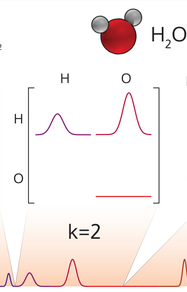
\includegraphics[width=0.9\linewidth]{theme/images/mbtr_with_k.png}
            \caption{MBTR}
            \label{fig:placeholder}
        \end{figure}
    \end{column}
\end{columns}

\end{frame}

\begin{frame}{$n_{grid}$ Correlation Score Evaluation}
\begin{columns}[T]

% Left column: text/formula
\begin{column}{0.55\textwidth}
\[
C_2 = \sum_{j=1}^{n}\left|\sum_{i=1}^{k} \mathrm{Corr}\left(MBTR^{(i)}, SASA\right)\right|
\]
\begin{itemize}
    \item We use SASA correlation because SASA is our target variable — the property MBTR ultimately needs to predict.
    \item $n$: number of configurations
    \item $k = 2$: interaction order
    \item Objective: maximize correlation between MBTR features and SASA
\end{itemize}
\end{column}

% Right column: table
\begin{column}{0.55\textwidth}
\begin{table}[]
    \centering
    \small
    \begin{tabular}{|c|c|c|}
    \hline
    \rowcolor{gray}
         $n_{grid}$ & Features & Mean Corr. \\
         \hline
         2 & 12 & \textbf{0.3956} \\
         \hline
         3 & 18 & 0.3777 \\
         \hline
         4 & 24 & 0.3145 \\
         \hline
         5 & 30 & 0.3309 \\
         \hline
         6 & 36 & 0.3368 \\
         \hline
         7 & 42 & 0.3204 \\
         \hline
         8 & 48 & 0.3301 \\
         \hline
         9 & 54 & 0.3279 \\
         \hline
         10 & 60 & 0.3209 \\
         \hline
         50 & 300 & 0.3287 \\
         \hline
         100 & 600 & 0.3295 \\
         \hline
    \end{tabular}
    \caption{Correlation to SASA. Max in bold.}
    \label{tab:ngrid_correlation}
\end{table}
\end{column}

\end{columns}
\end{frame}

\begin{frame}{SASA Extraction}
SASA is the surface traced by the center of a solvent probe (typically a water molecule) as it rolls over a molecule's van der Waals surface, measuring how exposed each part of the molecule is to solvent.\\

%HF: Solvent Accessible Surface Area (SASA) is the surface traced by the center of a solvent probe (typically representing a water molecule) as it rolls over the van der Waals surface of a molecule. 
% Measure exposure to solvent

SASA is extracted using the \textbf{MDTraj} library:
\begin{itemize}
    \item Library: MDTraj
    \item Method: Shrake--Rupley algorithm
    \item Probe radius: 0.14 nm
    \item Sphere discretization: 960 points
\end{itemize}
\end{frame}

\begin{frame}{SASA vs Time}
    \begin{figure}
        \centering
        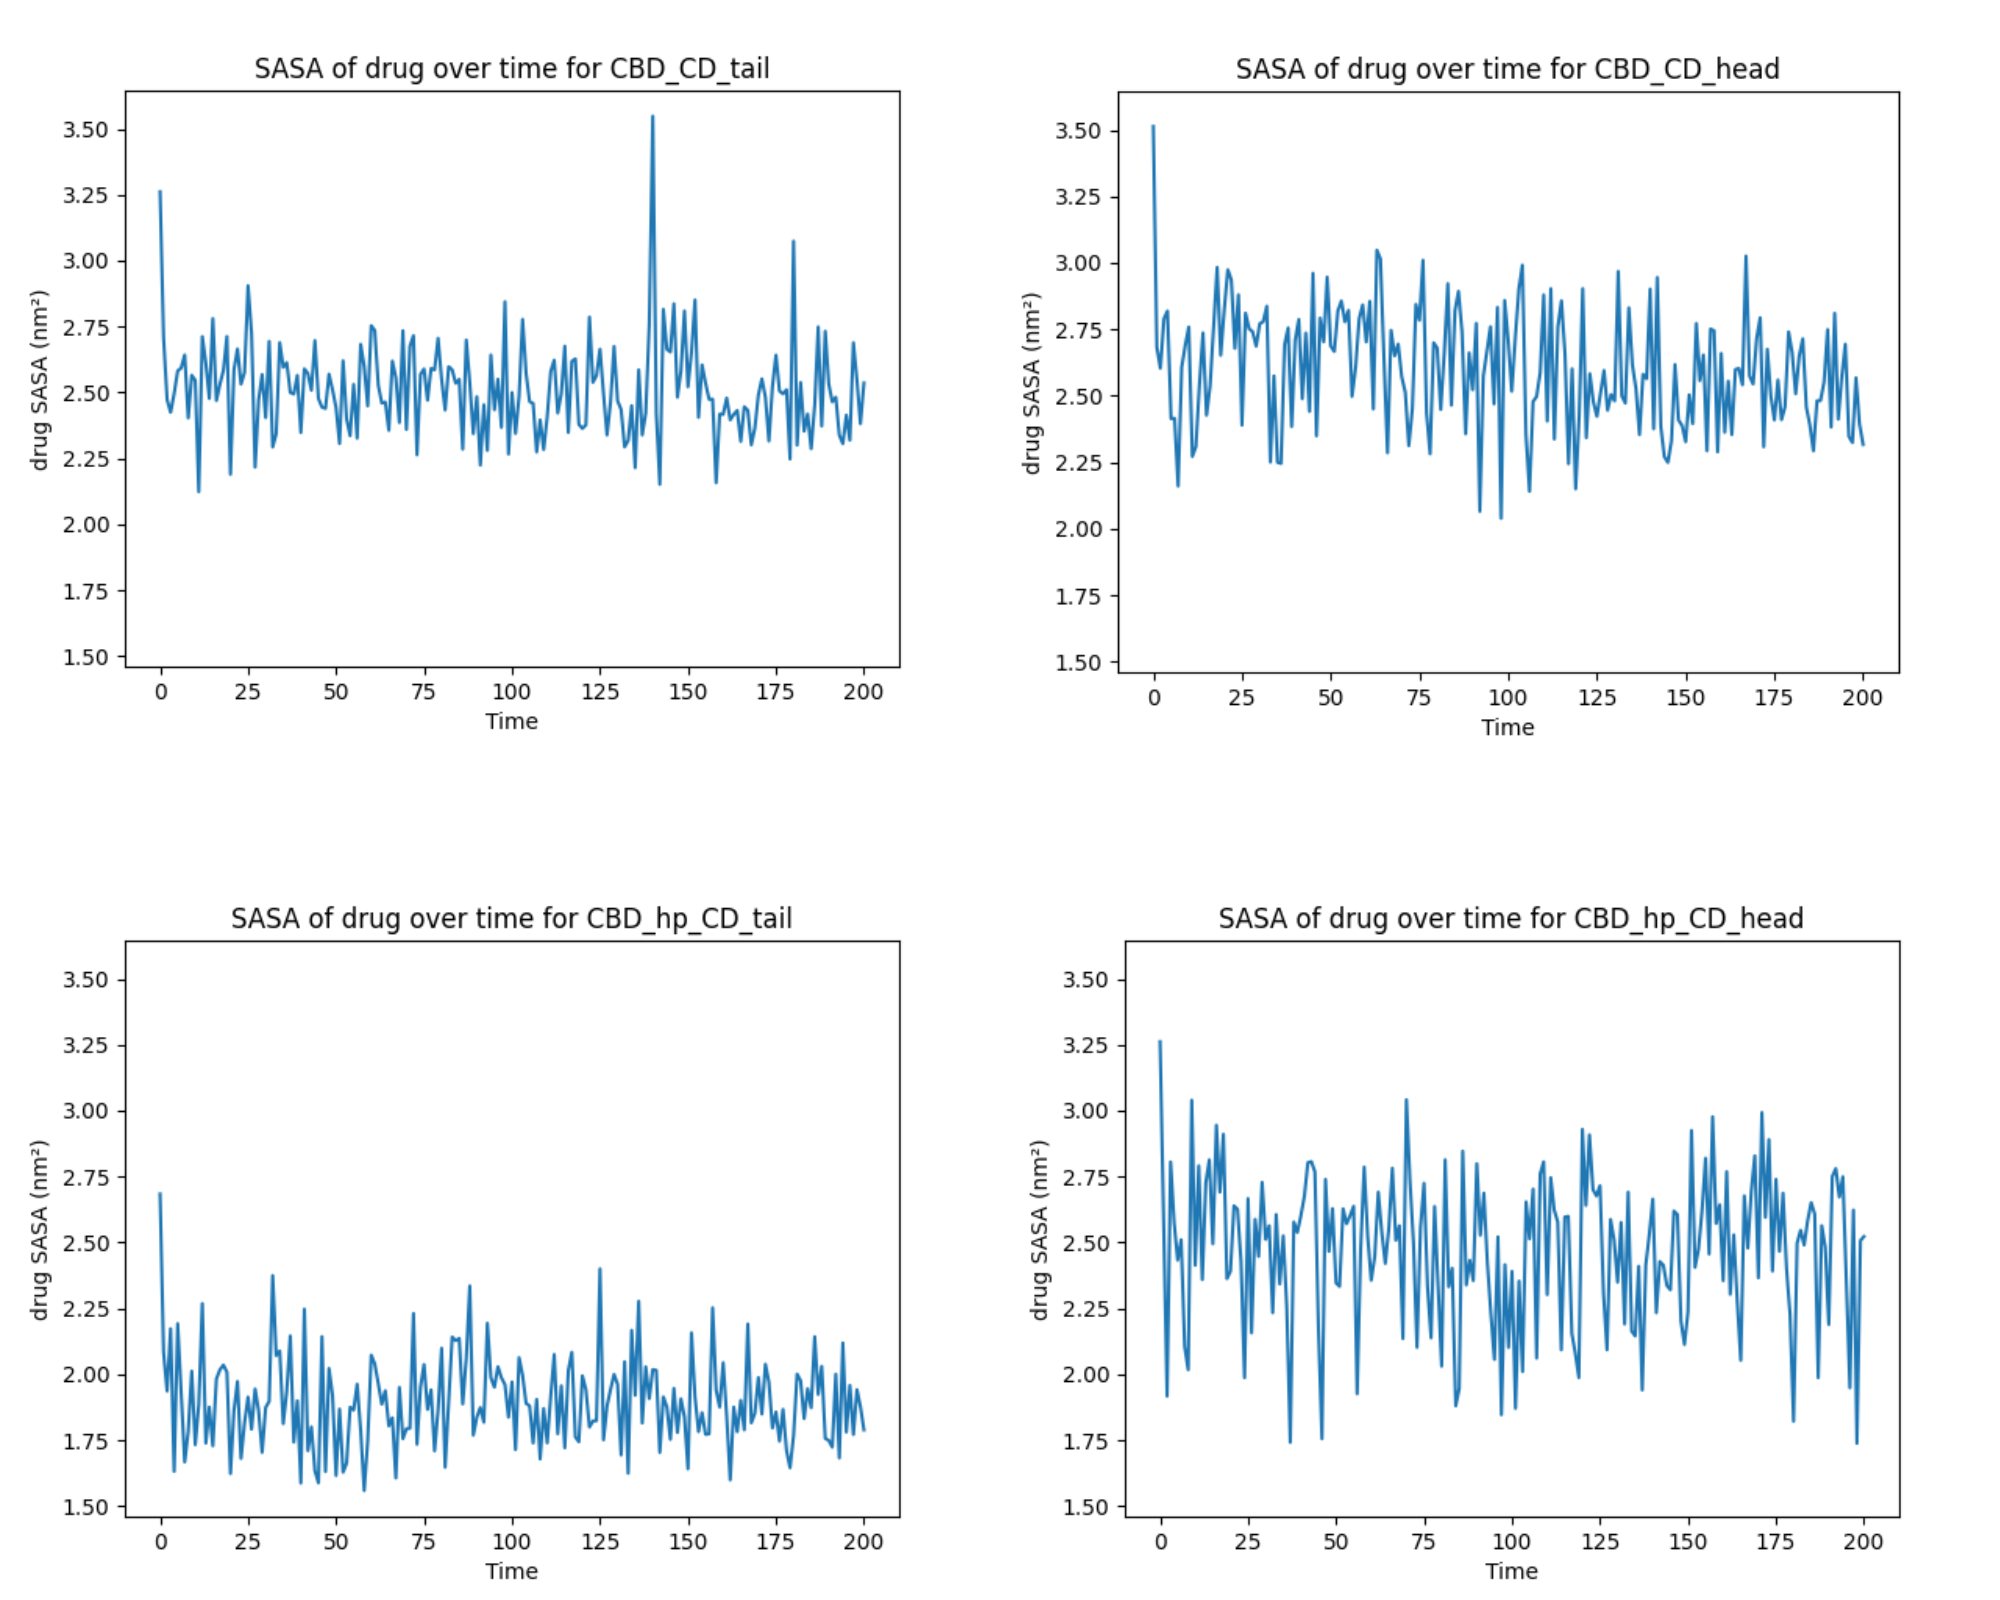
\includegraphics[width=12cm, height =6cm]{theme/images/sasa_time.png}
        \caption{SASA evolution over time for all 4 CD--CBD complex systems}
        \label{fig:sasa_time}
    \end{figure}
\end{frame}

\begin{frame}{Dataset Construction \& Preprocessing}
\begin{itemize}
    \item \textbf{Dataset Construction:}
    \begin{itemize}
        \item MBTR feature vectors combined per system, with a \textbf{System Name} identifier column
        \item All systems merged into a single unified dataset
    \end{itemize}
    \vspace{0.2cm}
    \item \textbf{Train/Val/Test Splitting:}
    \begin{itemize}
        \item 8:1:1 split, performed independently per system
    \end{itemize}
    \vspace{0.2cm}
    \item \textbf{Window Size Optimization:}
    \begin{itemize}
        \item Tested window sizes: $\{2,...,10,\ 50,\ 100\}$
        \item Selected via \textbf{grid search}, evaluated using Mean Squared Error (MSE) on validation set
        \item Two training strategies compared:
        \begin{itemize}
            \item \textbf{Per-system:} one model trained per system, scores averaged across systems
            \item \textbf{Pooled:} one model trained on all systems combined, scored on pooled validation set
        \end{itemize}
    \end{itemize}
\end{itemize}
\end{frame}

\begin{frame}{Time Series Model}
 \begin{figure}[htbp]
    \centering
    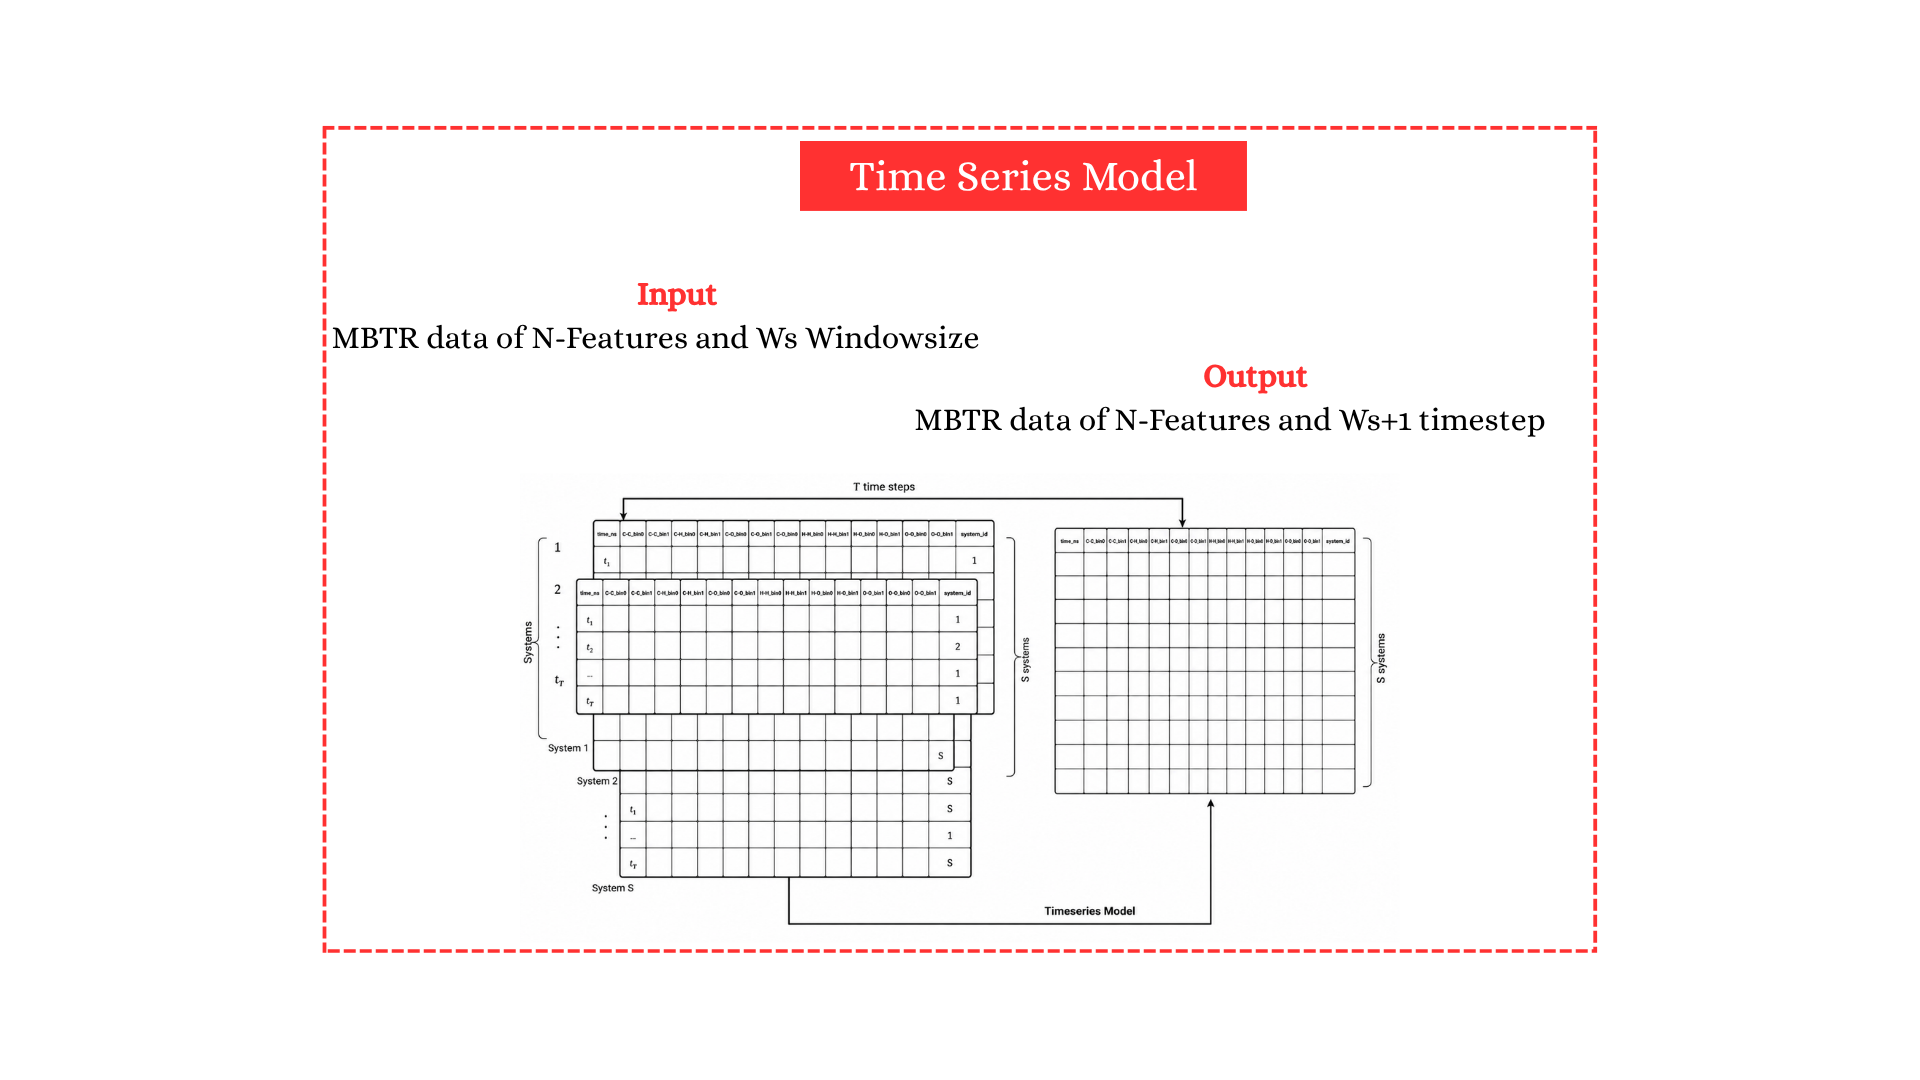
\includegraphics[width=0.85\textwidth]{theme/images/time_series_model.png}
    \caption{Time Series Modeling}
    \label{fig:time-series-model}
\end{figure}
\end{frame}


\begin{frame}{Machine Learning Models}
\begin{center}
    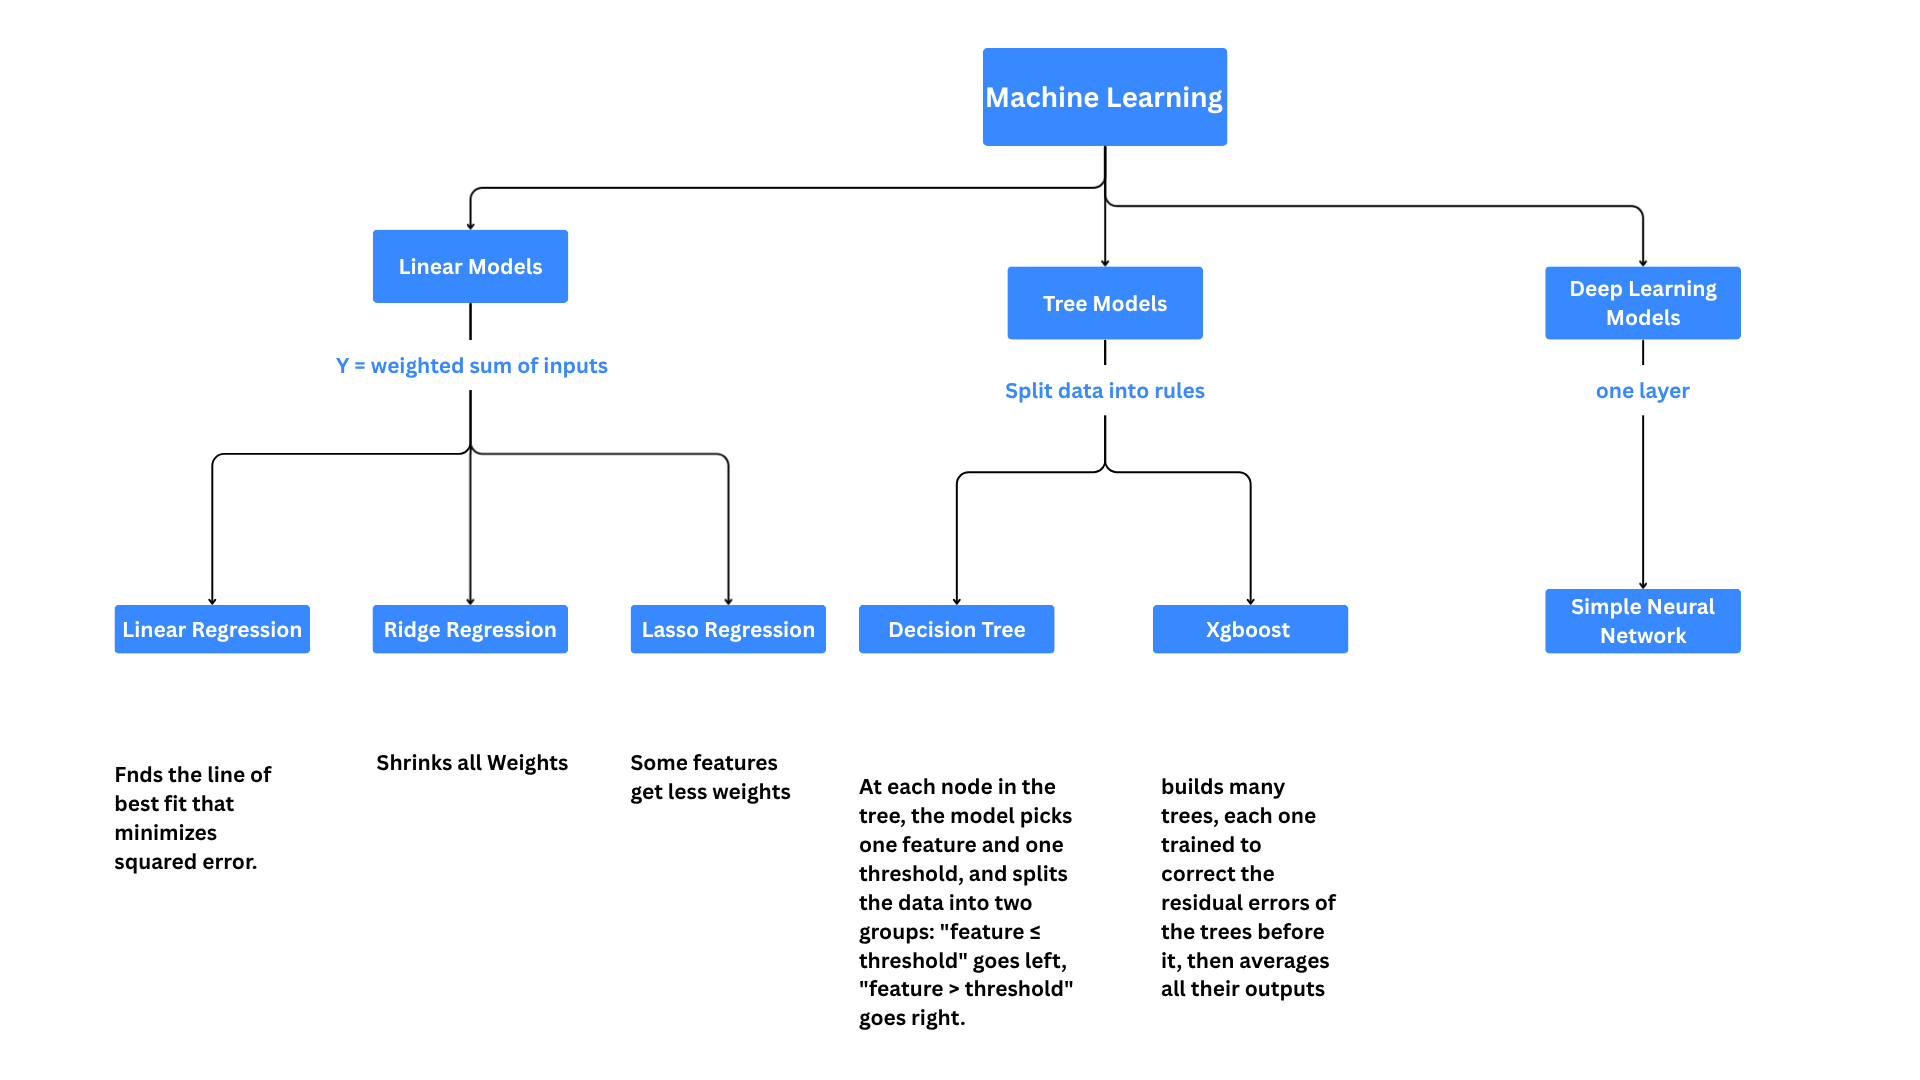
\includegraphics[width=0.85\linewidth]{theme/images/Machine Learning.png}
\end{center}
\end{frame}

\begin{frame}{Linear Models}
\begin{table}[h]
\centering
\resizebox{6.8cm}{!}{
\begin{tabular}{|l|c|c|c|}
\hline
\textbf{Model} & \textbf{Window Size} & \textbf{Val MSE (Per System)} & \textbf{Val MSE (Combined)} \\
\hline
Linear Regression & 2  & \textbf{0.9963} & 0.1712 \\
 & 4  & 1.2397 & 0.1665 \\
 & 6  & 1.6742 & 0.1610 \\
 & 8  & 2.4515 & 0.1638 \\
 & 10 & 4.8884 & 0.1766 \\
 & 12 & 40.4245 & 0.1800 \\
 & 14 & 22.4145 & \textbf{0.1317} \\
 & 16 & 8.0949 & 0.1471 \\
 & 18 & 5.5307 & 0.1559 \\
 \hline
 Ridge Regression & 2 & \textbf{1.0001} & 0.1688 \\
 & 4 & 1.1018 & 0.1619  \\
& 6  & 1.3562 & 0.1548 \\
 & 8 & 1.6961 & 0.1552  \\
 & 10  & 2.1599 & 0.1631 \\
 & 12 & 2.4290 & 0.1729  \\
 & 14 & 1.7767 & 0.1215  \\
 & 16 & 2.6682 & \textbf{0.1188 } \\
& 18 & 2.8743 & 0.1314  \\
\hline
Lasso Regression & 2  & 1.0320 & 0.9390 \\
& 4  & 1.0390 & 0.9295 \\
 & 6  & 1.0438 & 0.9395 \\
 & 8  & 1.0838 & 0.9348 \\
 & 10 & 1.1038 & 0.9465 \\
& 12 & 1.1582 & 0.9641 \\
& 14 & 0.9548 & 0.9102 \\
& 16 & \textbf{0.7357 } &\textbf{0.8905}  \\
& 18 & 0.8120 & 0.9662 \\
\hline
\end{tabular}
}

\caption{Validation MSE for Linear,Ridge and Lasso across different window sizes.}
\label{tab:lr_val_mse}
\end{table}
\end{frame}

\begin{frame}{Decision Tree}

\begin{table}[h]
\centering
\begin{tabular}{|l|c|c|c|}
\hline
\textbf{Window Size} & \textbf{Val MSE (Per System)} & \textbf{Val MSE (Combined)} \\
\hline
2  & $1.1582 \times 10^{-5}$ & $1.1749 \times 10^{-5}$ \\
4  & $1.1333 \times 10^{-5}$ & $1.1048 \times 10^{-5}$ \\
6  & $1.0833 \times 10^{-5}$ & $9.1487 \times 10^{-6}$ \\
8  & $1.1353 \times 10^{-5}$ & $1.1605 \times 10^{-5}$ \\
10 & $1.2431 \times 10^{-5}$ & $1.7244 \times 10^{-5}$ \\
12 & $1.1642 \times 10^{-5}$ & $8.7959 \times 10^{-6}$ \\
14 & $\mathbf{7.7868 \times 10^{-6}}$ & $8.7675 \times 10^{-6}$ \\
16 & $9.4837 \times 10^{-6}$ &  $\mathbf{6.3069 \times 10^{-6}}$ \\
18 & $1.9458 \times 10^{-5}$ & $6.6697 \times 10^{-6}$ \\
\hline
\end{tabular}
\caption{Validation MSE for Decision Tree across different window sizes.}
\label{tab:dt_val_mse}
\end{table}

\end{frame}

\begin{frame}{Xgboost}
\begin{table}[h]
\centering
\begin{tabular}{|l|c|c|c|}
\hline
\textbf{Window Size} & \textbf{Val MSE (Per System)} & \textbf{Val MSE (Combined)} \\
\hline
2  & $6.8269 \times 10^{-6}$ & $9.6230 \times 10^{-6}$ \\
4  & $6.0303 \times 10^{-6}$ & $9.4017 \times 10^{-6}$ \\
6  & $5.8109 \times 10^{-6}$ & $6.0319 \times 10^{-6}$ \\
8  & $5.8779 \times 10^{-6}$ & $5.9628 \times 10^{-6}$ \\
10 & $5.7993 \times 10^{-6}$ & $5.7370 \times 10^{-6}$ \\
12 & $5.9237 \times 10^{-6}$ & $6.3332 \times 10^{-6}$ \\
14 & $4.0527 \times 10^{-6}$ & $4.5747 \times 10^{-6}$ \\
16 & $\mathbf{3.7264 \times 10^{-6}}$ & $\mathbf{4.0499 \times 10^{-6}}$ \\
18 & $4.2176 \times 10^{-6}$ & $4.1780 \times 10^{-6}$ \\
\hline
\end{tabular}
\caption{Validation MSE for XGBoost across different window sizes.}
\label{tab:xgb_val_mse}
\end{table}
\end{frame}

\begin{frame}{Simple Neural Network}
    \begin{table}[h]
\centering
\begin{tabular}{|l|c|c|c|}
\hline
\textbf{Window Size} & \textbf{Val MSE (Per System)} & \textbf{Val MSE (Combined)} \\
\hline
2  & 0.9342 & 0.1708 \\
4  & 0.8671 & 0.1627 \\
6  & 0.9116 & 0.1595 \\
8  & 0.8888 & 0.1592 \\
10 & 0.8959 & 0.1564 \\
12 & 0.9542 & 0.1166 \\
14 & 0.7252 & 0.1058 \\
16 & 0.6408 & \textbf{0.0754} \\
18 & \textbf{0.5505 }& 0.0819 \\
\hline
\end{tabular}
\caption{Validation MSE for Simple Neural Network across different window sizes.}
\label{tab:nn_val_mse}
\end{table}

\end{frame}
\begin{frame}{Model Comparison}
\begin{table}[h]
\centering
\resizebox{14.5cm}{!}{
\begin{tabular}{|l|c|c|c|c|}
\hline
\textbf{Model Name} & \textbf{Window Size (Per-Sys.)} & \textbf{Test MSE (Per-Sys.)} & \textbf{Window Size (Combined)} & \textbf{Test MSE (Combined)} \\
\hline
Linear Regression & 2  & 0.1265 & 14 & 0.1676 \\
Ridge Regression  & 2  & 0.1254 & 16 & 0.1587 \\
Lasso Regression  & 16 & 0.8565 & 16 & 0.8565 \\
Decision Tree      & 14 & $8.1968 \times 10^{-6}$ & 16 & $1.0259 \times 10^{-5}$ \\
XGBoost            & 16 & $4.5596 \times 10^{-6}$ & 16 & $4.5596 \times 10^{-6}$ \\
Neural Network    & 18 & 0.0771 & 16 & 0.1093 \\
\hline
\end{tabular}
}

\caption{Model comparison: best window size and Test MSE, per-system vs. combined.}
\label{tab:model_comparison_merged}
\end{table}
    
\end{frame}

\begin{frame}{SASA Model}
    \begin{figure}
        \centering
        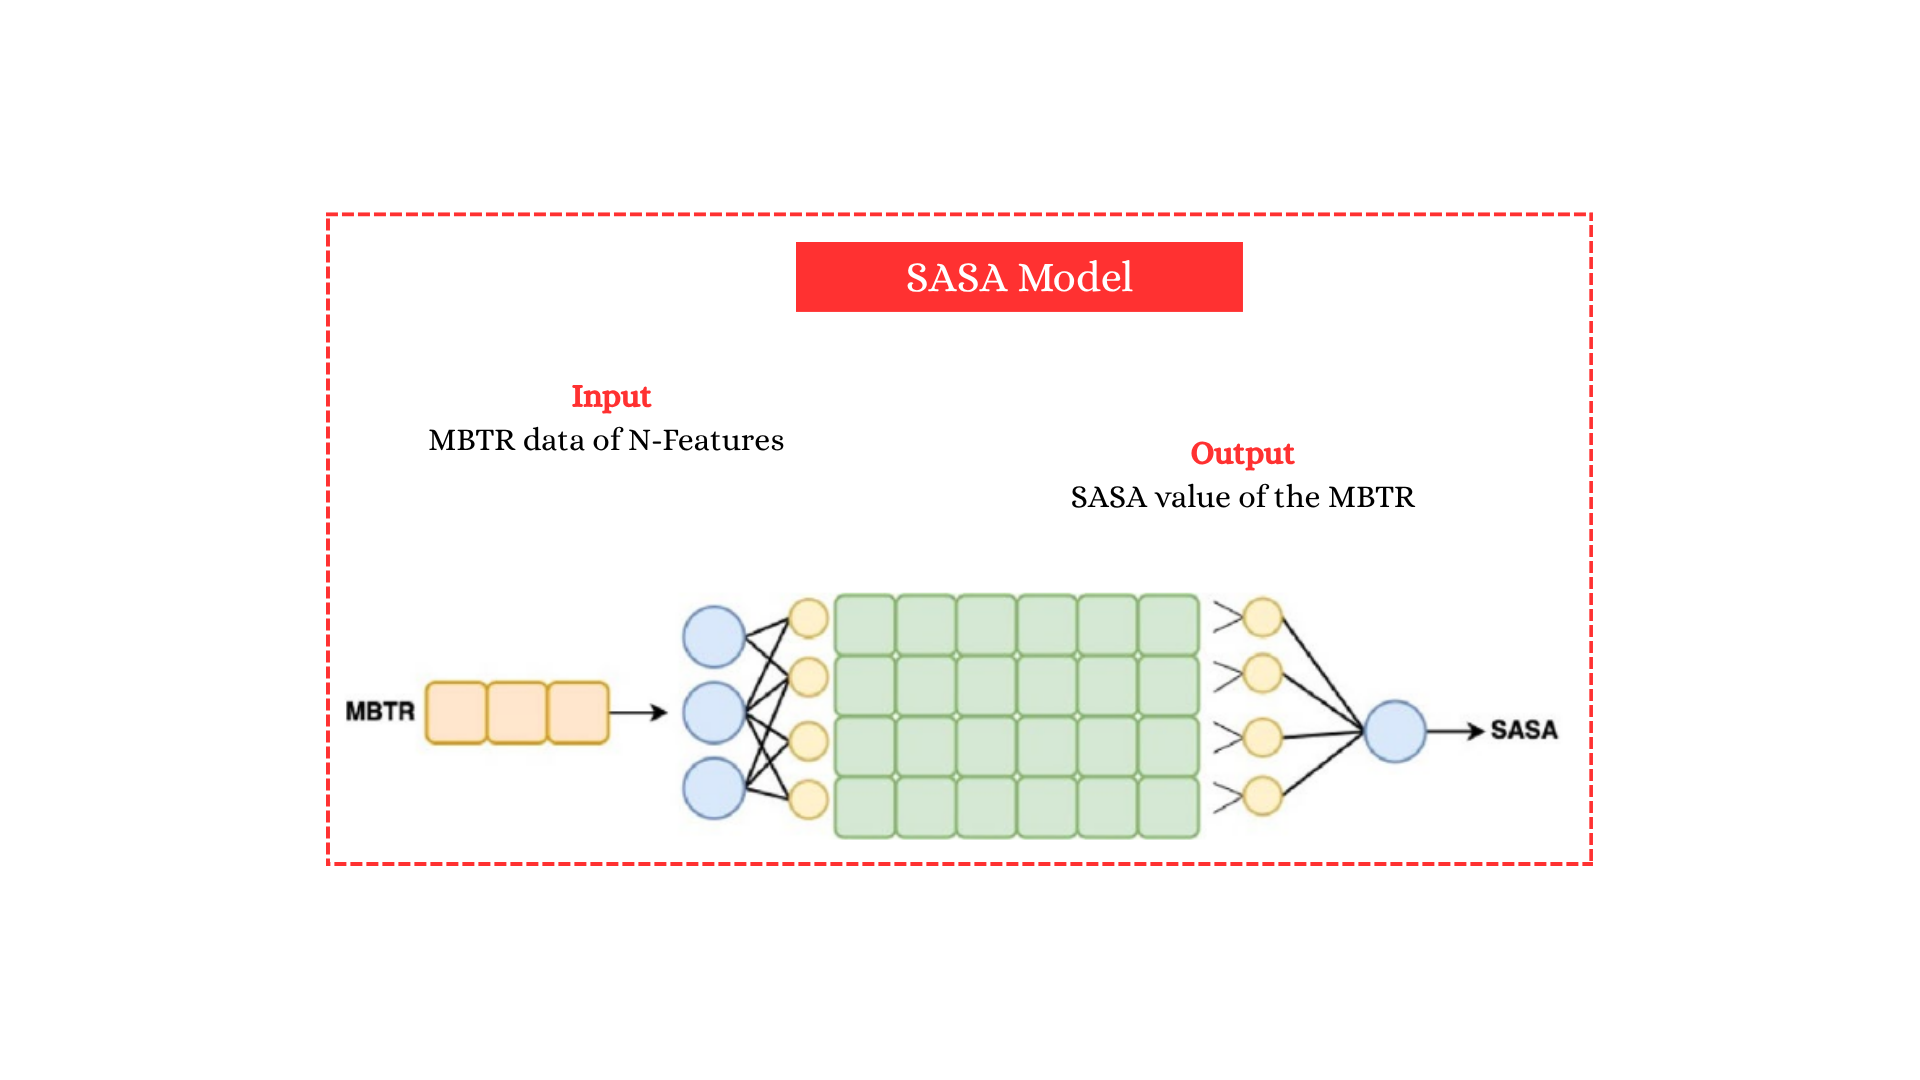
\includegraphics[width=0.85\linewidth]{theme/images/sasa_model.png}
        \caption{SASA Model}
        \label{fig:placeholder}
    \end{figure}
\end{frame}

\begin{frame}{Linear Model}
\begin{table}[h]
\centering
\resizebox{10cm}{!}{
\begin{tabular}{|l|c|}
\hline
\textbf{System} & \textbf{MAE} \\
\hline
CBD\_CD\_tail    & 0.0733 \\
CBD\_CD\_head    & 0.0948 \\
CBD\_hp\_CD\_tail & 0.1024 \\
CBD\_hp\_CD\_head & 0.1382 \\

\hline
\end{tabular}
}

\caption{Mean Absolute Error (MAE) by system.}
\label{tab:mae_by_system}
\end{table}
    
\end{frame}

\begin{frame}{Challenges \& Future Work}
    \textbf{Challenges}
    \begin{itemize}
        \item Limited data availability
    \end{itemize}
    \vspace{0.5cm}
    \textbf{Future Work}
    \begin{itemize}
        \item Increase the amount of data per system
        \item Hyperparameter Optimization
        \item Training on different feature 
        \item Add models such as Elastic Net
        \item Train on different/additional feature sets
        \item Extend prediction to other properties (orientation, center of 
              gravity)
    \end{itemize}
\end{frame}

\end{document}
